\documentclass[a4paper,oneside,12pt]{extreport}

\usepackage{mmap}
\usepackage[T2A]{fontenc}
\usepackage[utf8]{inputenc}
\usepackage[english,russian]{babel}

\usepackage[left=30mm, right=15mm, top=20mm, bottom=20mm]{geometry}

\setlength{\parindent}{1.25cm} % Абзацный отступ

\usepackage{setspace}
\onehalfspacing % Полуторный интервал

\frenchspacing % Равномерные пробелы
\usepackage{indentfirst} % Красная строка

\usepackage{microtype}
\sloppy

\usepackage{titlesec}
\titlespacing*{\chapter}{0pt}{-30pt}{8pt}
\titlespacing*{\section}{\parindent}{*4}{*4}
\titlespacing*{\subsection}{\parindent}{*4}{*4}
\titleformat{\chapter}{\LARGE\bfseries}{\thechapter}{20pt}{\LARGE\bfseries}
\titleformat{\section}{\Large\bfseries}{\thesection}{40pt}{\Large\bfseries}

\usepackage{graphicx}
\usepackage{caption}

\usepackage[unicode,pdftex]{hyperref}
\hypersetup{hidelinks}

\usepackage{amsmath}

%% title begin
\usepackage{wrapfig}

\makeatletter
	\def\vhrulefill#1{\leavevmode\leaders\hrule\@height#1\hfill \kern\z@}
\makeatother
%% title end

%% begin code
\usepackage{listings}
\usepackage{xcolor}

\lstset{
	basicstyle=\footnotesize\ttfamily,
	breakatwhitespace=true,
	breaklines=true,
	commentstyle=\color{gray},
	frame=single,
	keywordstyle=\color{blue},
	stringstyle=\color{red},
	tabsize=8
}

\newcommand{\code}[1]{\texttt{#1}}
%% end code


\begin{document}

\begin{titlepage}
	{\large % 14pt instead of 12pt
	\onehalfspacing
	\centering

	\begin{wrapfigure}[7]{l}{0.14\linewidth}
		\vspace{3mm}
		\hspace{-10mm}
		
\includegraphics[width=0.93\linewidth]{inc/img/bmstu-logo}
	\end{wrapfigure}
	{\singlespacing \footnotesize \bfseries Министерство науки и высшего образования Российской Федерации\\Федеральное государственное бюджетное образовательное учреждение\\высшего образования\\<<Московский государственный технический университет\\имени Н.~Э.~Баумана\\ (национальный исследовательский университет)>>\\(МГТУ им. Н.~Э.~Баумана)\\}

	\vspace{-2.2mm}
	\vhrulefill{0.9mm}\\
	\vspace{-7.5mm}
	\vhrulefill{0.2mm}\\
	\vspace{2mm}

	{\doublespacing \small \raggedright ФАКУЛЬТЕТ \hspace{37mm} «Информатика и системы управления»\\
	КАФЕДРА \hspace{17mm} «Программное обеспечение ЭВМ и информационные технологии»\\}

	\vspace{30mm}

	\textbf{ОТЧЁТ}\\
	По лабораторной работе № 2\\
	По курсу: «Моделирование»\\
	Тема: «Распределение случайных величин»\\
	Вариант: 6 $\equiv$ 2 (mod 4)\\

	\vspace{40mm}

	\begin{flushleft}
		\begin{tabular}{lr}
			\textbf{Студент:}        & Керимов~А.~Ш. \\
			\textbf{Группа:}         & ИУ7-74Б       \\
			\textbf{Оценка (баллы):} & \hrulefill    \\
			\textbf{Преподаватель:}  & Рудаков~И.~В. \\
		\end{tabular}
	\end{flushleft}

	\vfill

	Москва\\
	\the\year\\}
\end{titlepage}

\setcounter{page}{2}


Дан колебательный контур с газоразрядной трубкой

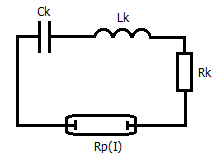
\includegraphics{inc/img/scheme}

Получена система дифференциальных уравнений:
\begin{equation*}
	\left\{
	\begin{aligned}
		L_k & \frac{\mathrm dI}{\mathrm dt} + (R_k + R_p) I - U_c = 0, \\
		C_k & \frac{\mathrm dU_c}{\mathrm dt} = -I.
	\end{aligned}
	\right.
\end{equation*}

Даны таблицы зависимостей $T_0$ и $m$ от $I$, $\sigma$ от $T$.

Требуется построить графики зависимостей $I(t)$, $R_p(t)$, $U_c(t)$, $U_p(t)$.

Сопротивление газоразрядной трубки находится в зависимости от силы тока:
\begin{equation*}
	R_p(I) = \frac{l_\text{э}}{2 \pi R^2 \int_0^1 \sigma(T(z))z\,\mathrm dz}.
\end{equation*}

Система уравнений решается методом Рунге-Кутта 4-го порядка:
\begin{equation*}
	\begin{aligned}
		y_{n+1} &= y_n + \frac{k_1 + 2k_2 + 2k_3 + k_4}{6},\\
		z_{n+1} &= z_n + \frac{q_1 + 2q_2 + 2q_3 + q_4}{6},
	\end{aligned}
\end{equation*}
где
\begin{equation*}
	\begin{aligned}
		&k_1  = h_n f(x_n, y_n, z_n),
		&q_1 &= h_n g(x_n, y_n, z_n), \\
		&k_2  = h_n f(x_n + \frac{h_n}{2}, y_n + \frac{k_1}{2}, z_n + \frac{q_1}{2}),
		&q_2 &= h_n g(x_n + \frac{h_n}{2}, y_n + \frac{k_1}{2}, z_n + \frac{q_1}{2}), \\
		&k_3  = h_n f(x_n + \frac{h_n}{2}, y_n + \frac{k_2}{2}, z_n + \frac{q_2}{2}),
		&q_3 &= h_n g(x_n + \frac{h_n}{2}, y_n + \frac{k_2}{2}, z_n + \frac{q_2}{2}), \\
		&k_4  = h_n f(x_n + h_n, y_n + k_3, z_n + q_3),
		&q_4 &= h_n g(x_n + h_n, y_n + k_3, z_n + q_3). \\
	\end{aligned}
\end{equation*}

\lstinputlisting[caption={Интерполяция}, style=cpp, linerange={91-112}]{../solve.cpp}

\lstinputlisting[caption={Интегрирование}, style=cpp, linerange={114-131}]{../solve.cpp}

\lstinputlisting[caption={Решение системы ОДУ}, style=cpp, linerange={137-177}]{../solve.cpp}

\end{document}
